\chapter{Incertezza nelle decisioni mediche}
\label{cap:incertezza-decisioni-mediche}

In quest'era di medicina di precisione e di medicina predittiva, le incertezze che i medici devono affrontare sono sorprendentemente vaste, ben oltre le aspettative di una società che crede in una scienza moderna infallibile. Nonostante i progressi significativi nel campo della ricerca biomedica, i medici spesso si trovano a dover fare scelte basate su dati non completi e su una comprensione parziale di certe malattie. La medicina si trova a navigare in un mare di variabili aleatorie e incertezze, una realtà difficile da accettare per i pazienti, i quali cercano risposte chiare e sicure riguardo alla loro salute attuale e futura.\\
La realtà è che in sanità l'incertezza non è un'eccezione ma una costante. Questa condizione viene descritta come l'incapacità di prendere decisioni a causa di una percezione soggettiva dell'ignoranza, definita come "meta-ignoranza"\footcite{womak:meta-ignoranza}. Spesso, l'ignoranza è considerata inaccettabile in ambito sanitario, che richiede certezze e prove inequivocabili per formulare previsioni accurate e decisioni professionali prive di dubbi. Di conseguenza, i professionisti sanitari possono sviluppare atteggiamenti di avversione o negazione dell'incertezza, cercando rifugio in false certezze.\\
Diviene quindi complesso per i medici comunicare queste sfumature, poiché potrebbe sembrare che ammettere la presenza di incertezza minacci la loro affidabilità. La responsabilità dei medici non è solo quella di gestire il rischio, ma anche di supportare i pazienti nel comprendere e accettare l'incertezza relativa alle loro condizioni cliniche.

\section{Definizione}

Ma cosa si intende per incertezza? L'incertezza è un termine che assume diversi significati in vari ambiti del sapere. Etimologicamente parlando, la parola certezza deriva dal verbo latino "cernere", che significa separare, distinguere. "Certum", il participio passato di "cernere", indica qualcosa di separato, distinto e chiaramente delimitato\footcite{womak:recenti-progressi-medicina}. Al contrario, le circostanze incerte sono quelle che non sono chiaramente distinguibili o separabili. Non sorprende quindi che l'incertezza venga definita come incapacità di prendere decisioni. Questa incapacità può essere attribuita ai fatti e alla realtà o può riguardare il soggetto. Han et al. hanno definito l'incertezza come una "meta-ignoranza"\footcite{womak:meta-ignoranza}, ovvero la percezione soggettiva dell'ignoranza. In questa accezione, l'incertezza non è nella realtà, ma è un fenomeno cognitivo, emotivo e comportamentale che si manifesta nel soggetto incerto attraverso una serie di fenomeni cognitivi\footcite{womak:recenti-progressi-medicina} e affettivi, tra cui:

\begin{itemize}
    \item Dubbio;
    \item Percezione di indefinito;
    \item Percezione di indeterminazione;
    \item Sensazione di non essere credibili;
    \item Ansia;
    \item Comportamenti di evitamento dell'incertezza (ambiguity aversion);
\end{itemize}

\noindent Secondo Han sono almeno tre livelli di incertezza (\ref{fig:fonti-incertezza}). Il primo tipo di incertezza è quello scientifico, che deriva dalle informazioni con cui il professionista si confronta per prendere decisioni. L'incertezza è legata all'indeterminatezza degli eventi futuri, spesso espressa in termini percentuali di probabilità. Questa incertezza è misurabile e fornisce una guida utile per il decisore. Il grado di incertezza aumenta se le informazioni disponibili sono ambigue, ovvero non univoche, inaffidabili o difficili da interpretare\footcite{womak:recenti-progressi-medicina}. Cresce ulteriormente quando le informazioni sono complesse, con molteplici fattori causali, stati di eventi, esiti o interpretazioni possibili, e quando i confini tra eventi sono vaghi o difficili da descrivere.\\
Un secondo tipo di incertezza è di natura pratico-organizzativa\footcite{womak:recenti-progressi-medicina}, poiché qualsiasi intervento diagnostico o terapeutico dipende dalla qualità del sistema sanitario in cui è inserito.\\
Infine, l'incertezza può derivare dalle informazioni fornite dal paziente stesso sulla propria salute e sulla sua rete di assistenza. Questo è particolarmente rilevante nelle cure primarie, dove quasi tutti gli interventi iniziano dalla soggettività del paziente.\\

\begin{figure}[!ht] 
    \centering 
    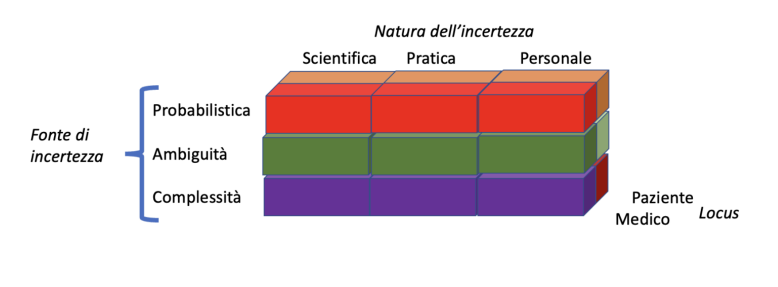
\includegraphics[width=0.9\columnwidth]{fonti-incertezza} 
    \caption{Natura e fonti dell'incertezza secondo Han et al.}
    \label{fig:fonti-incertezza}
\end{figure}

Le situazioni cliniche possono quindi essere descritte come costituite da un nucleo di rischio, con probabilità di esito noto, circondato da una "nuvola" di incertezza, che diventa più ampia quanto più vaga e imprecisa è l'informazione clinica disponibile\footcite{womak:clinica-relazione-decisione}. Questa nuvola di incertezza deve essere sempre considerata, poiché influisce significativamente sulle probabilità degli esiti.


\section{Metodologia e valutazione del rischio nella pratica clinica}

Il ragionamento clinico è fondamentale in medicina per affrontare qualsiasi situazione. Oggi, si riconosce che l'approccio del medico alla situazione clinica non si basa solo su modelli analitici, consci e controllati dal ragionamento, ma anche su modelli non analitici, inconsci e intuitivi. L'insegnamento del metodo clinico raccomandato, quindi, include entrambe queste tipologie. Quando non è possibile affidarsi a un dato numerico o statistico, i medici si affidano a quella che viene chiamata \textit{gut feeling}\footcite{womak:arte-probabilita-coen}, oppure all'euristica\footcite{womak:recenti-progressi-medicina}.\\
In queste occasioni, è la sensazione del medico a indicare qual è la decisione giusta da prendere; c'è una sorta di consapevolezza fisica su quale sarebbe la decisione giusta, senza ragionarci troppo sopra.\\
Questa sensazione in realtà non è solo un'intuizione, è soprattutto un'attivazione del sistema nervoso enterico, che è composto da milioni di neuroni collegati al nostro intestino. L'euristica somiglia al gut feeling perché non è sempre razionale. Si basa sull'identificazione di poche informazioni importanti, vengono valutate e si interrompe la ricerca quando si ritiene che queste informazioni siano sufficienti per una decisione adeguata.

La conclusione è che il percorso diagnostico del medico si alterna tra euristiche, ragionamento deduttivo, e confronto con altri\footcite{womak:arte-probabilita-coen}. Tuttavia non sono le uniche opzioni disponibili per i medici; tra le strategie decisionali rapide ma basate su evidenze vi sono le cosiddette \textit{\gls{clinical-decision-rules}} o \textit{\gls{clinical-prediction-rules}}, in cui pochi segni e sintomi, insieme a esami \textit{\gls{point-of-care}} \footcite{womak:recenti-progressi-medicina}, possono essere utilizzati per prendere rapidamente una decisione clinica.

Gigerenzer dimostra\footcite{womak:gigerenzer-euristiche} come nelle situazioni di rischio conosciuto, i sistemi di decisione basati sull'analisi delle probabilità siano i migliori, mentre nelle situazioni di incertezza, le strategie euristiche rapide dei professionisti abbiano maggiore successo. Questo approccio si basa sull'idea che, in molte situazioni della vita reale, le risorse cognitive (come il tempo e l'informazione completa) sono limitate, e quindi le persone devono fare affidamento su metodi di decisione che siano efficienti in termini di risorse. In medicina, quindi, in molti casi, le strategie rapide possono essere più efficaci di quelle basate esclusivamente su metodi analitici. Utilizzare strategie euristiche evita anche di aumentare le indagini diagnostiche in situazioni di incertezza.\\

Nella pratica clinica, i medici si confrontano quotidianamente con informazioni probabilistiche per prendere decisioni\footcite{womak:arte-probabilita-coen}. Esempi includono stime di sopravvivenza alla malattia in ambito oncologico, valutazione del rischio cardiovascolare, e la probabilità di eziologia batterica o virale in infezioni respiratorie. L'incertezza che ne deriva è legata all'indeterminatezza degli eventi futuri, spesso espressa in percentuali di probabilità\footcite{womak:recenti-progressi-medicina}. Questa incertezza è misurabile e fornisce una guida utile al decisore, ma non è eliminabile, poiché rimane una previsione probabilistica e non deterministica.\\
Nelle situazioni più ambigue e con esiti incerti, è cruciale valutare attentamente il ruolo della consulenza specialistica e la gestione condivisa del caso, che possono ridurre l'incertezza a livelli accettabili per il paziente. Tuttavia, è importante riconoscere che un certo grado di incertezza sarà sempre presente e dovrà essere gestito attraverso una comunicazione chiara e trasparente con il paziente.


\section{Rapporto con il paziente}

Comunicare le incertezze al paziente è fondamentale per costruire un percorso decisionale consapevole. Nonostante la medicina moderna si basi su numeri e analisi statistiche di  esperienze pregresse, presupponendo che ogni opzione diagnostica o terapeutica sia la più appropriata, la comunicazione del medico trasmette non solo logica, ma anche significato, influenzando la percezione del paziente e le sue aspettative. È essenziale che la comunicazione delle incertezze non confonda ulteriormente il paziente, ma che si adatti alle sue caratteristiche individuali (età, cultura, fattori psicologici) sia nella complessità dell'informazione che nel linguaggio utilizzato.\\
%  È certo però che dal punto di vista del paziente l'ignoranza dei medici riguardo queste aree di incertezza può indurre una diffidenza che non aiuta la comunicazione tra le parti. \\

Le situazioni cliniche possono essere rappresentate come formate da un corpo centrale di rischio conosciuto, affrontabile con la conoscenza probabilistica, circondato da una nube di incertezza(\ref{fig:incertezza-situazioni-cliniche}). La gestione dell'incertezza in medicina non dovrebbe limitarsi a una semplice ricognizione anamnestica, ma deve essere un aspetto chiave del metodo clinico, incorporato in tutti gli aspetti del processo decisionale dei professionisti sanitari. Questo è essenziale per attuare azioni appropriate.\\

\begin{figure}[!ht] 
    \centering 
    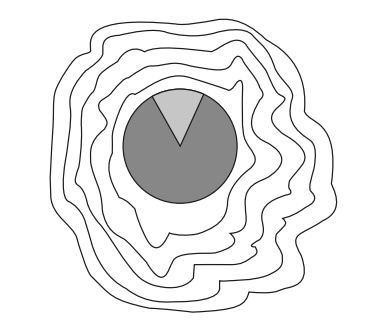
\includegraphics[width=0.5\columnwidth]{incertezza-situazioni-cliniche} 
    \caption{Illustrazione di come si configurano le situazioni cliniche}
    \caption*{La parte in grigio scuro rappresenta il rischio in percentuale che un evento si verifichi; il grigio chiaro rappresenta il rischio in percentuale che un evento non si verifichi; le linee circolari intorno rappresentano la nube di incertezza}
    \label{fig:incertezza-situazioni-cliniche}
\end{figure}


Nel processo decisionale clinico, l'incertezza influisce sulla probabilità che un evento si verifichi o meno. Riconoscere l'incertezza consente di comunicarla, prendere decisioni più consapevoli e praticare una medicina più prudente e meno onnipotente.
In base alle preferenze espresse dal paziente, è possibile costruire una rete protettiva (safety netting) adottando una strategia di attesa. Vengono descritti al paziente una serie di sintomi di allarme (red flags) \footcite{womak:recenti-progressi-medicina} potenzialmente riscontrabili e i tempi e le modalità per cercare aiuto medico se questi sintomi si manifestassero o se non ci fossero miglioramenti in un periodo prestabilito. Idealmente, queste informazioni dovrebbero essere fornite per iscritto, dopo un processo decisionale condiviso.\\

Esistono situazioni in cui la diagnosi è incerta e l'alternativa potrebbe essere una malattia grave a progressione rapida. In questi casi, si può utilizzare il tempo come forma di test, simile a un esame ematico o strumentale\footcite{womak:recenti-progressi-medicina} \footcite{womak:strategie-nella-diagnostica}. In questo caso l'aspetto comunicativo della strategia è cruciale, perchè il medico deve creare una buona relazione di fiducia e collaborazione con il paziente, affinché quest'ultimo possa comprendere chiaramente le istruzioni. Il paziente, inoltre, deve essere consapevole dell'incertezza diagnostica, dei segni e sintomi a cui prestare attenzione e del periodo di osservazione, nonché sapere come cercare aiuto\footcite{womak:arte-probabilita-coen}.\\
È fondamentale anche l'aspetto organizzativo: il medico e il suo team devono avere accesso alle informazioni sulla decisione presa con il paziente in ogni momento, e deve esistere un sistema di ricezione delle chiamate che preveda una risposta immediata.\\
In generale comunque i risultati non sono sempre chiari, di fatto lo strumento più potente per aiutare il medico a decidere nell'incertezza è la condivisione del processo decisionale con il paziente o con chi se ne prende cura.\\

Al giorno d'oggi il paziente può influire sul processo decisionale in medicina. Kon sostiene che la decisione condivisa esiste su un continuum con il modello paternalistico (guidato dal medico) a un'estremità e il modello informativo (guidato dal paziente) all'altra, mentre al centro c'è la \textit{decisione condivisa}\footcite{womak:decisione-condivisa-kon} in cui medico e paziente contribuiscono equamente, ciascuno al 50\%.\\


\begin{figure}[!ht] 
    \centering 
    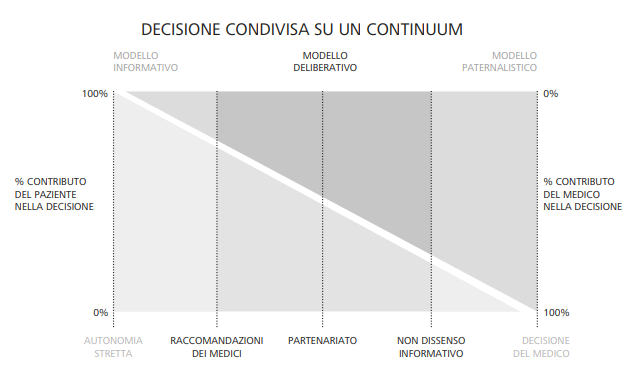
\includegraphics[width=0.9\columnwidth]{decisione-condivisa-kon} 
    \caption{Modello della decisione condivisa secondo Kon}
\end{figure}

Occorre considerare quale situazione clinica richiede un maggiore coinvolgimento del paziente. Questa è spesso una situazione di incertezza, contrapposta a una in cui esiste una chiara opzione migliore con un rapporto costi/benefici ben definito. In contesti incerti, le preferenze e i valori del paziente diventano cruciali poiché non ci sono rapporti chiari tra costi e benefici. Più è grande l'incertezza, più è necessario coinvolgere il paziente, valutando le sue conoscenze e capacità. Questo non significa solo considerare le preferenze, ma anche integrare il contributo del paziente nella decisione.\\

È importante distinguere la decisione condivisa dal semplice consenso informato\footcite{womak:recenti-progressi-medicina}: quest'ultimo implica un flusso informativo unidirezionale dal medico al paziente, che è eticamente e legalmente obbligatorio ma non necessariamente parte di una decisione già presa dal medico. La vera decisione condivisa implica invece uno scambio di idee tra medico e paziente, una collaborazione che porta a una decisione comune. In questo processo, il paziente agisce come consulente, aiutando il medico a prendere una decisione, il che è molto diverso da un semplice processo informativo.

